% Options for packages loaded elsewhere
\PassOptionsToPackage{unicode}{hyperref}
\PassOptionsToPackage{hyphens}{url}
\documentclass[
  ignorenonframetext,
]{beamer}
\newif\ifbibliography
\usepackage{pgfpages}
\setbeamertemplate{caption}[numbered]
\setbeamertemplate{caption label separator}{: }
\setbeamercolor{caption name}{fg=normal text.fg}
\beamertemplatenavigationsymbolsempty
% remove section numbering
\setbeamertemplate{part page}{
  \centering
  \begin{beamercolorbox}[sep=16pt,center]{part title}
    \usebeamerfont{part title}\insertpart\par
  \end{beamercolorbox}
}
\setbeamertemplate{section page}{
  \centering
  \begin{beamercolorbox}[sep=12pt,center]{section title}
    \usebeamerfont{section title}\insertsection\par
  \end{beamercolorbox}
}
\setbeamertemplate{subsection page}{
  \centering
  \begin{beamercolorbox}[sep=8pt,center]{subsection title}
    \usebeamerfont{subsection title}\insertsubsection\par
  \end{beamercolorbox}
}
% Prevent slide breaks in the middle of a paragraph
\widowpenalties 1 10000
\raggedbottom
\AtBeginPart{
  \frame{\partpage}
}
\AtBeginSection{
  \ifbibliography
  \else
    \frame{\sectionpage}
  \fi
}
\AtBeginSubsection{
  \frame{\subsectionpage}
}
\usepackage{iftex}
\ifPDFTeX
  \usepackage[T1]{fontenc}
  \usepackage[utf8]{inputenc}
  \usepackage{textcomp} % provide euro and other symbols
\else % if luatex or xetex
  \usepackage{unicode-math} % this also loads fontspec
  \defaultfontfeatures{Scale=MatchLowercase}
  \defaultfontfeatures[\rmfamily]{Ligatures=TeX,Scale=1}
\fi
\usepackage{lmodern}
\ifPDFTeX\else
  % xetex/luatex font selection
\fi
% Use upquote if available, for straight quotes in verbatim environments
\IfFileExists{upquote.sty}{\usepackage{upquote}}{}
\IfFileExists{microtype.sty}{% use microtype if available
  \usepackage[]{microtype}
  \UseMicrotypeSet[protrusion]{basicmath} % disable protrusion for tt fonts
}{}
\makeatletter
\@ifundefined{KOMAClassName}{% if non-KOMA class
  \IfFileExists{parskip.sty}{%
    \usepackage{parskip}
  }{% else
    \setlength{\parindent}{0pt}
    \setlength{\parskip}{6pt plus 2pt minus 1pt}}
}{% if KOMA class
  \KOMAoptions{parskip=half}}
\makeatother
\usepackage{color}
\usepackage{fancyvrb}
\newcommand{\VerbBar}{|}
\newcommand{\VERB}{\Verb[commandchars=\\\{\}]}
\DefineVerbatimEnvironment{Highlighting}{Verbatim}{commandchars=\\\{\}}
% Add ',fontsize=\small' for more characters per line
\usepackage{framed}
\definecolor{shadecolor}{RGB}{248,248,248}
\newenvironment{Shaded}{\begin{snugshade}}{\end{snugshade}}
\newcommand{\AlertTok}[1]{\textcolor[rgb]{0.94,0.16,0.16}{#1}}
\newcommand{\AnnotationTok}[1]{\textcolor[rgb]{0.56,0.35,0.01}{\textbf{\textit{#1}}}}
\newcommand{\AttributeTok}[1]{\textcolor[rgb]{0.13,0.29,0.53}{#1}}
\newcommand{\BaseNTok}[1]{\textcolor[rgb]{0.00,0.00,0.81}{#1}}
\newcommand{\BuiltInTok}[1]{#1}
\newcommand{\CharTok}[1]{\textcolor[rgb]{0.31,0.60,0.02}{#1}}
\newcommand{\CommentTok}[1]{\textcolor[rgb]{0.56,0.35,0.01}{\textit{#1}}}
\newcommand{\CommentVarTok}[1]{\textcolor[rgb]{0.56,0.35,0.01}{\textbf{\textit{#1}}}}
\newcommand{\ConstantTok}[1]{\textcolor[rgb]{0.56,0.35,0.01}{#1}}
\newcommand{\ControlFlowTok}[1]{\textcolor[rgb]{0.13,0.29,0.53}{\textbf{#1}}}
\newcommand{\DataTypeTok}[1]{\textcolor[rgb]{0.13,0.29,0.53}{#1}}
\newcommand{\DecValTok}[1]{\textcolor[rgb]{0.00,0.00,0.81}{#1}}
\newcommand{\DocumentationTok}[1]{\textcolor[rgb]{0.56,0.35,0.01}{\textbf{\textit{#1}}}}
\newcommand{\ErrorTok}[1]{\textcolor[rgb]{0.64,0.00,0.00}{\textbf{#1}}}
\newcommand{\ExtensionTok}[1]{#1}
\newcommand{\FloatTok}[1]{\textcolor[rgb]{0.00,0.00,0.81}{#1}}
\newcommand{\FunctionTok}[1]{\textcolor[rgb]{0.13,0.29,0.53}{\textbf{#1}}}
\newcommand{\ImportTok}[1]{#1}
\newcommand{\InformationTok}[1]{\textcolor[rgb]{0.56,0.35,0.01}{\textbf{\textit{#1}}}}
\newcommand{\KeywordTok}[1]{\textcolor[rgb]{0.13,0.29,0.53}{\textbf{#1}}}
\newcommand{\NormalTok}[1]{#1}
\newcommand{\OperatorTok}[1]{\textcolor[rgb]{0.81,0.36,0.00}{\textbf{#1}}}
\newcommand{\OtherTok}[1]{\textcolor[rgb]{0.56,0.35,0.01}{#1}}
\newcommand{\PreprocessorTok}[1]{\textcolor[rgb]{0.56,0.35,0.01}{\textit{#1}}}
\newcommand{\RegionMarkerTok}[1]{#1}
\newcommand{\SpecialCharTok}[1]{\textcolor[rgb]{0.81,0.36,0.00}{\textbf{#1}}}
\newcommand{\SpecialStringTok}[1]{\textcolor[rgb]{0.31,0.60,0.02}{#1}}
\newcommand{\StringTok}[1]{\textcolor[rgb]{0.31,0.60,0.02}{#1}}
\newcommand{\VariableTok}[1]{\textcolor[rgb]{0.00,0.00,0.00}{#1}}
\newcommand{\VerbatimStringTok}[1]{\textcolor[rgb]{0.31,0.60,0.02}{#1}}
\newcommand{\WarningTok}[1]{\textcolor[rgb]{0.56,0.35,0.01}{\textbf{\textit{#1}}}}
\setlength{\emergencystretch}{3em} % prevent overfull lines
\providecommand{\tightlist}{%
  \setlength{\itemsep}{0pt}\setlength{\parskip}{0pt}}
\usepackage{graphicx}
\titlegraphic{\hfill
\includegraphics[height=1cm]{figures/tue.png}}
\usepackage{bookmark}
\IfFileExists{xurl.sty}{\usepackage{xurl}}{} % add URL line breaks if available
\urlstyle{same}
\hypersetup{
  pdftitle={An automated tool to improve scientific manuscripts},
  pdfauthor={Cristian Mesquida},
  hidelinks,
  pdfcreator={LaTeX via pandoc}}

\title{\texorpdfstring{An automated tool to improve scientific
manuscripts}{An automated tool to improve scientific manuscripts}}
\author{\texorpdfstring{Cristian Mesquida}{Cristian Mesquida}}
\date{2026-05-18}

\begin{document}
\frame{\titlepage}

\begin{frame}{}
\protect\phantomsection\label{section}
\begin{itemize}
\tightlist
\item
  The ISO-9001 framework provide standards for quality management
  systems in Human-Factors research and design
\end{itemize}
\end{frame}

\begin{frame}{}
\protect\phantomsection\label{section-1}
According to ISO-9001 framework, Organizations should: - establish
quality objectives - plan to achieve these objectives by considering the
resources required - For example support staff, infrastructure, and an
adequate social, psychological, and physical environment.
\end{frame}

\begin{frame}{}
\protect\phantomsection\label{section-2}
A crucial factor in ISO 9001:2015 is ensuring that people involved in
the work that is evaluated in quality management system are competent,
which means they have received the appropriate amount of education,
training, or experience.
\end{frame}

\begin{frame}{}
\protect\phantomsection\label{section-3}
\begin{itemize}
\tightlist
\item
  In science, this is unlikely to happen anytime soon
\item
  There is no quality management
\item
  Lack of time for training/education
\item
  Lack of expertise
\end{itemize}
\end{frame}

\begin{frame}{Some issues in published manuscripts}
\protect\phantomsection\label{some-issues-in-published-manuscripts}
\begin{itemize}
\tightlist
\item
  Invalid and unreliable measures
\item
  Misinterpretation of non-significant results
\item
  Vague preregistrations
\item
  Irreproducible and invalid a priori power analyses
\item
  Lack of adherence to reporting guidelines
\end{itemize}
\end{frame}

\begin{frame}{What can we do from a Human Factors perspective?}
\protect\phantomsection\label{what-can-we-do-from-a-human-factors-perspective}
Automatation
\end{frame}

\begin{frame}{Automatation}
\protect\phantomsection\label{automatation}
\begin{itemize}
\tightlist
\item
  In software development, automated checks are routinely used to
  identify issues before release
\item
  For example, CRAN checks for R packages
\item
  Before submitting a package to CRAN, a battery of tests must be passed
\end{itemize}
\end{frame}

\begin{frame}{CRAN checks}
\protect\phantomsection\label{cran-checks}
\begin{itemize}
\tightlist
\item
  Checking package namespace information \ldots{} OK
\item
  Checking package dependencies \ldots{} OK
\item
  Checking if this is a source package \ldots{} OK
\item
  Checking if there is a namespace \ldots{} OK
\item
  Checking for executable files \ldots{} OK
\end{itemize}
\end{frame}

\begin{frame}{}
\protect\phantomsection\label{section-4}
There is a number of tools that perform automated checks on scientific
manuscripts.
\end{frame}

\begin{frame}{Zotero}
\protect\phantomsection\label{zotero}
\begin{center}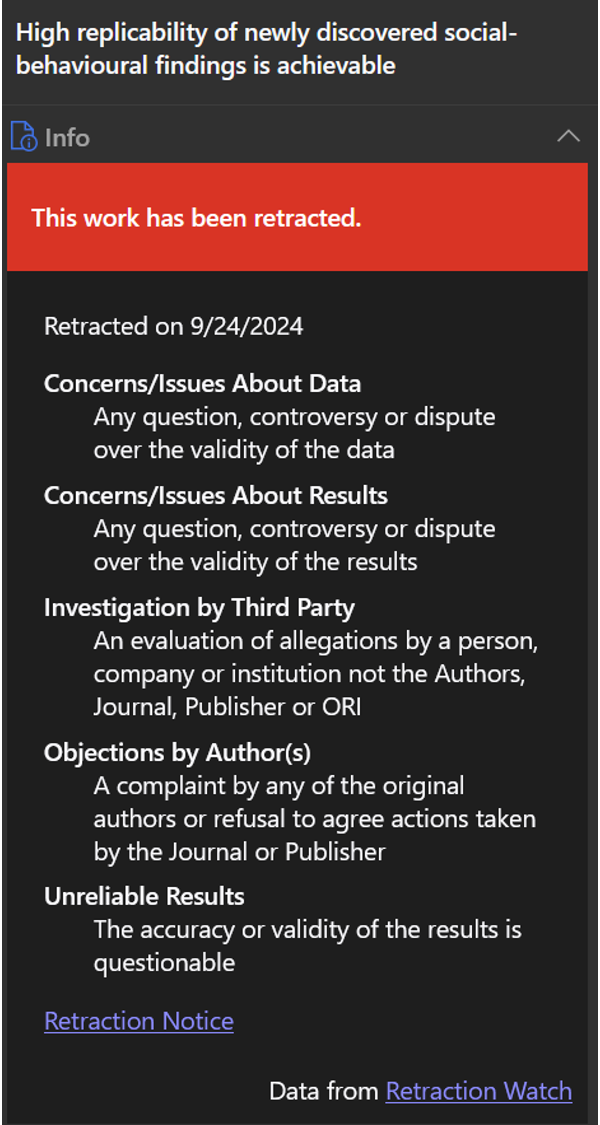
\includegraphics[width=0.5\linewidth]{figures/zotero} \end{center}
\end{frame}

\begin{frame}{}
\protect\phantomsection\label{section-5}
\begin{center}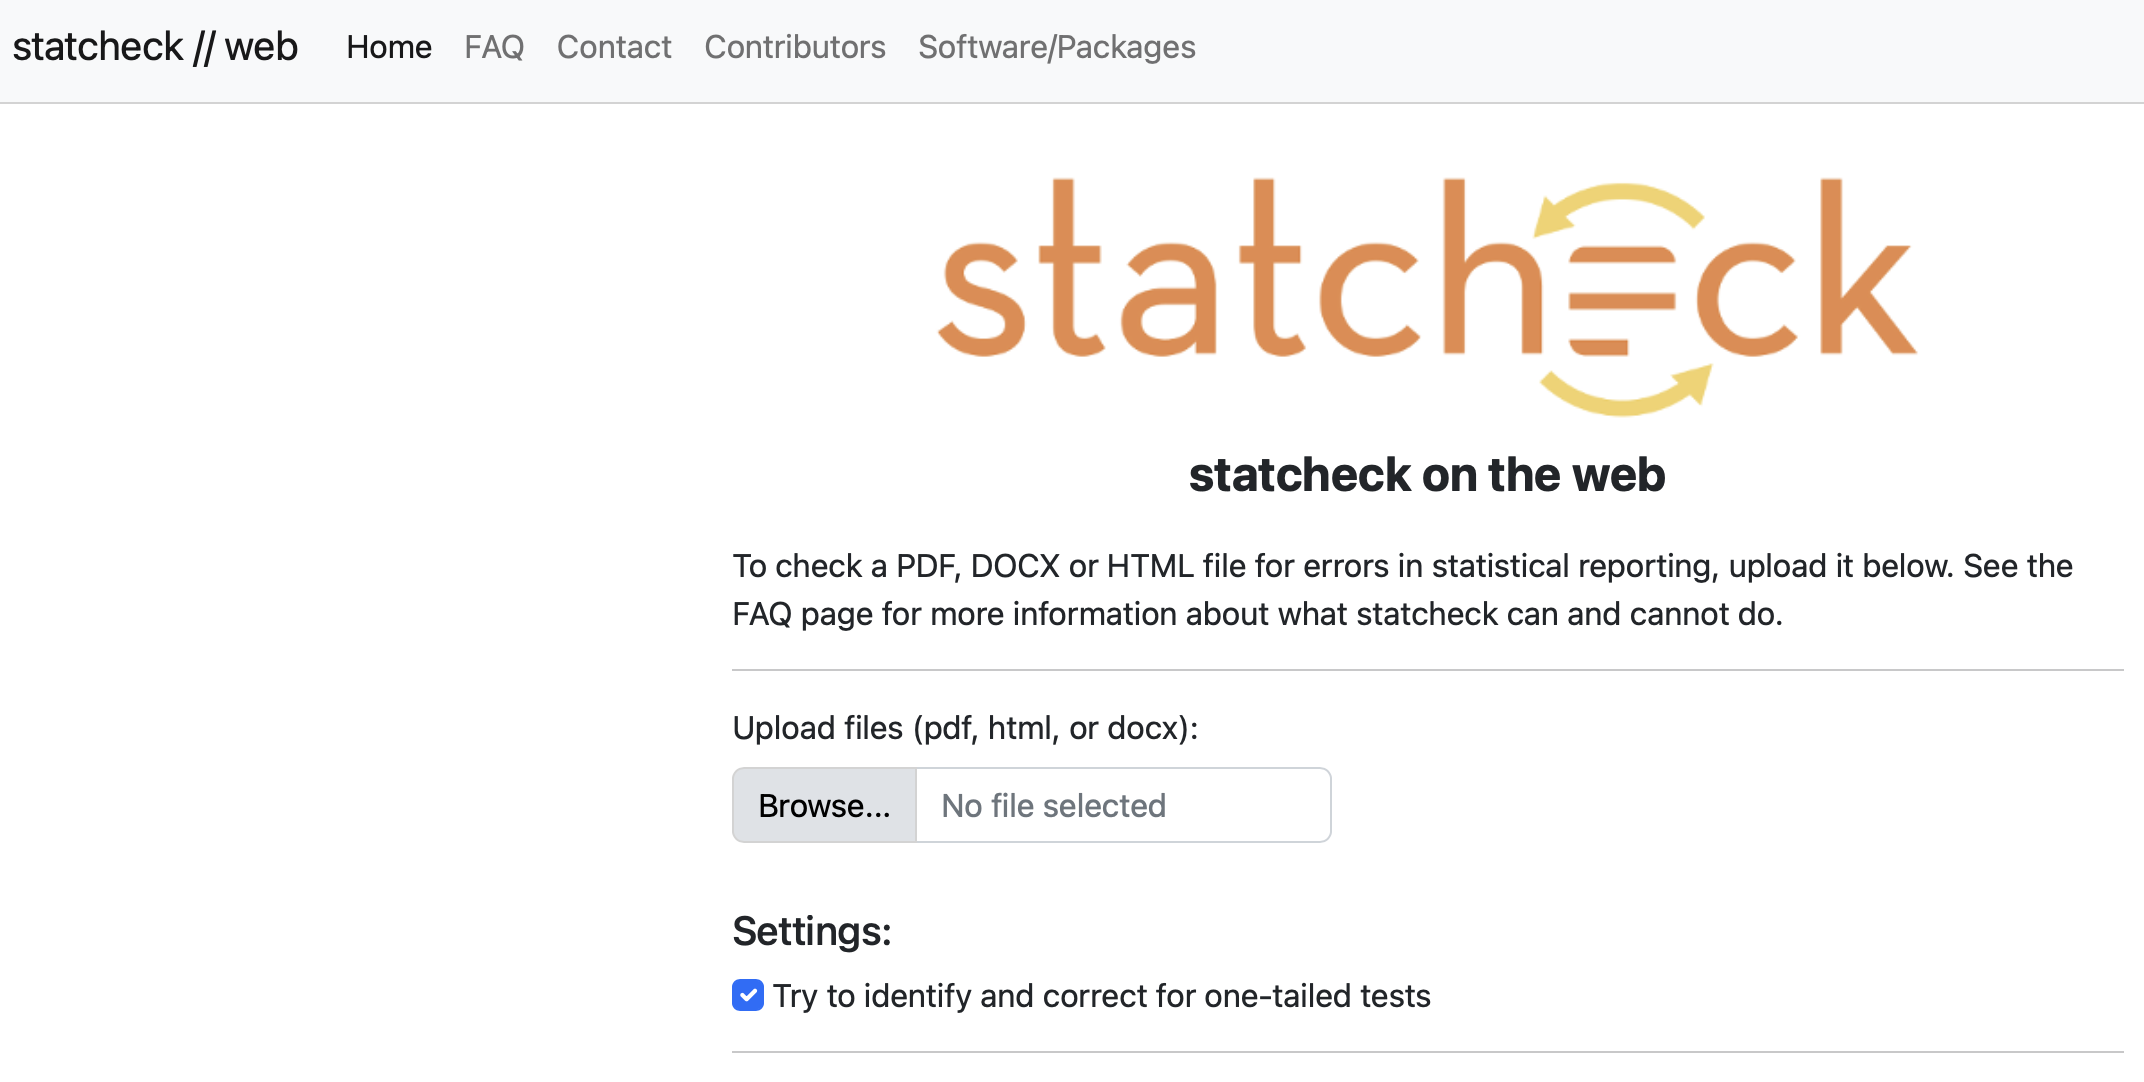
\includegraphics[width=0.8\linewidth]{figures/statcheck} \end{center}
\end{frame}

\begin{frame}{We are building Papercheck, an R package containing
modules to automate checks in manuscripts}
\protect\phantomsection\label{we-are-building-papercheck-an-r-package-containing-modules-to-automate-checks-in-manuscripts}
\begin{center}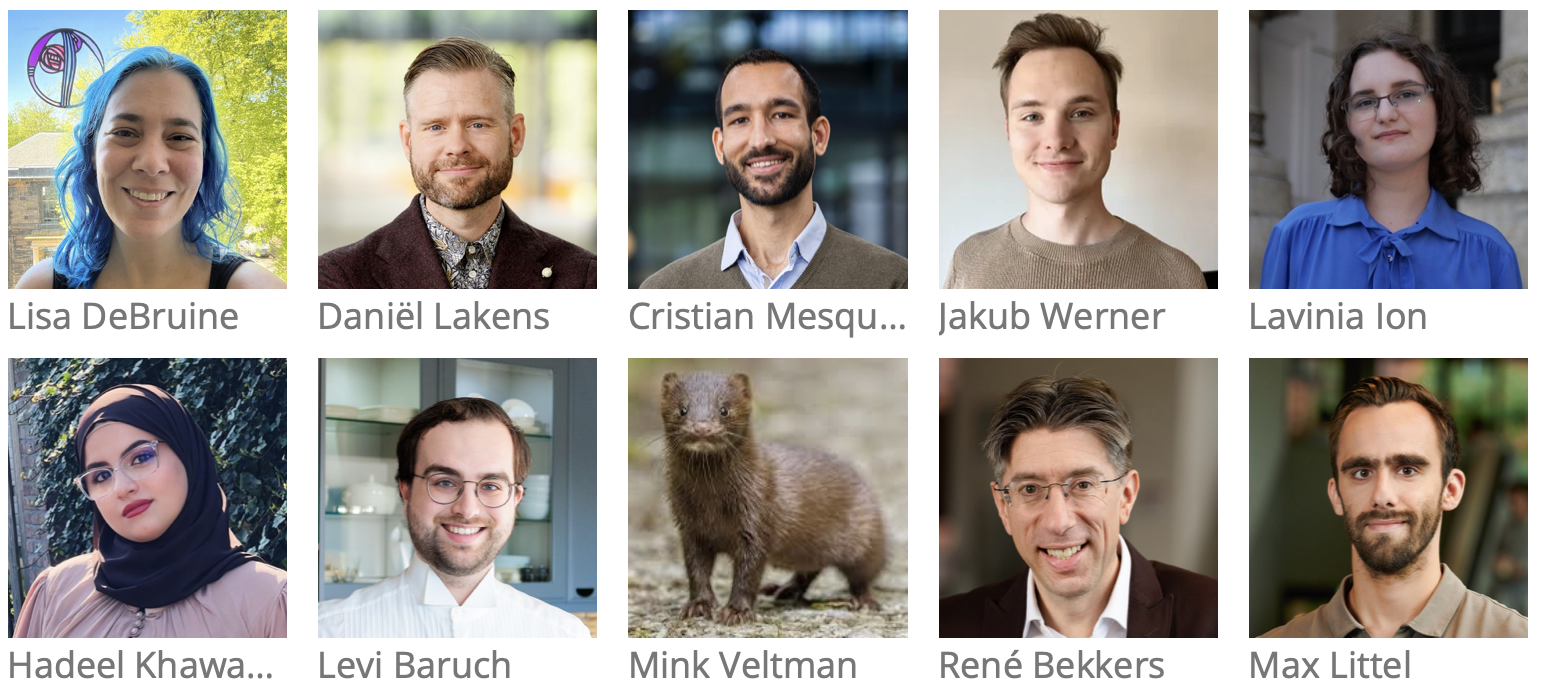
\includegraphics[width=0.8\linewidth]{figures/team} \end{center}
\end{frame}

\begin{frame}{Metacheck}
\protect\phantomsection\label{metacheck}
\begin{itemize}
\item
  An R package containing modules to automate checks in manuscripts
\item
  It leverages text search, code, and large language models to detect
  best practices or lack thereof in scientific manuscripts
\item
  It can be used in a single or multiple papers
\end{itemize}
\end{frame}

\begin{frame}{Workflow}
\protect\phantomsection\label{workflow}
\begin{center}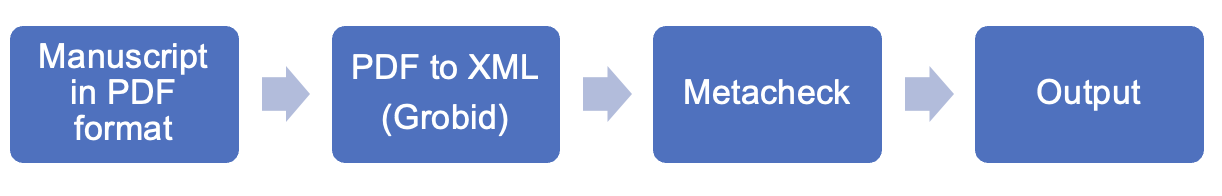
\includegraphics[width=0.8\linewidth]{figures/workflow} \end{center}
\end{frame}

\begin{frame}{Grobid}
\protect\phantomsection\label{grobid}
\begin{center}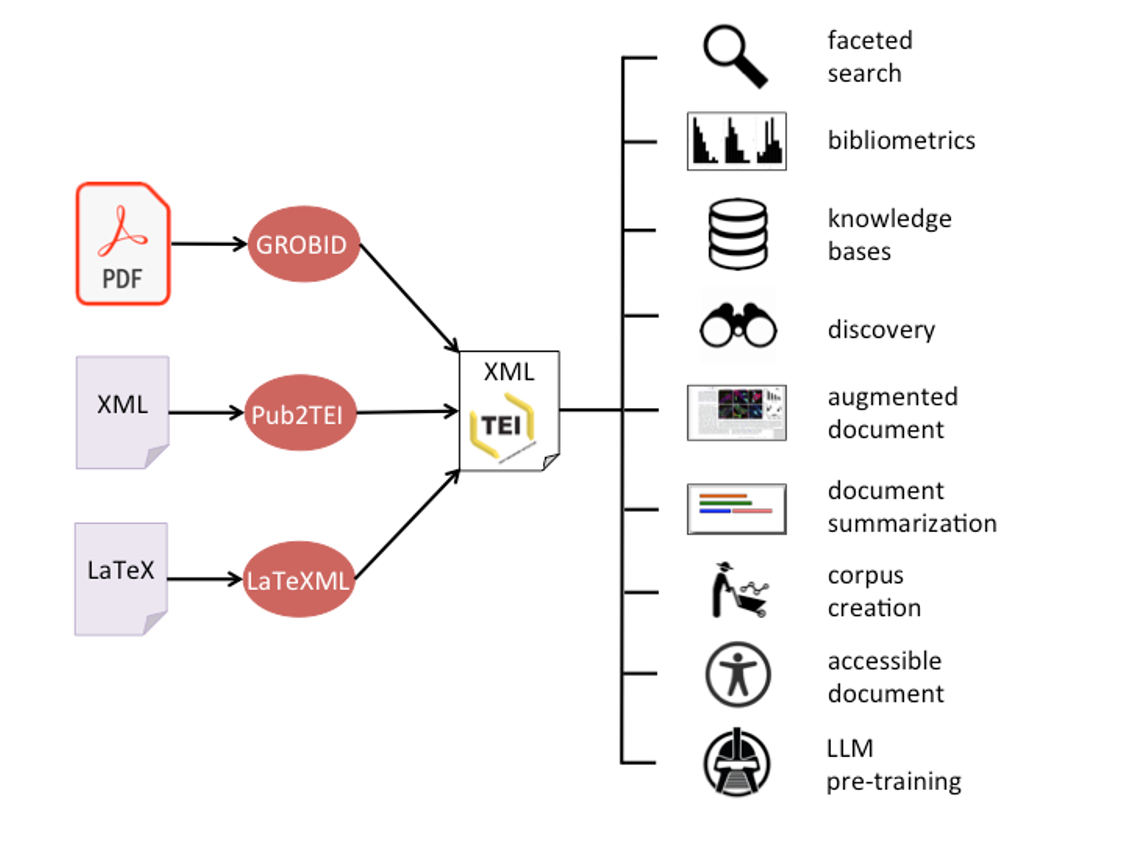
\includegraphics[width=0.8\linewidth]{figures/grobid} \end{center}
\end{frame}

\begin{frame}{Metacheck modules}
\protect\phantomsection\label{metacheck-modules}
\begin{center}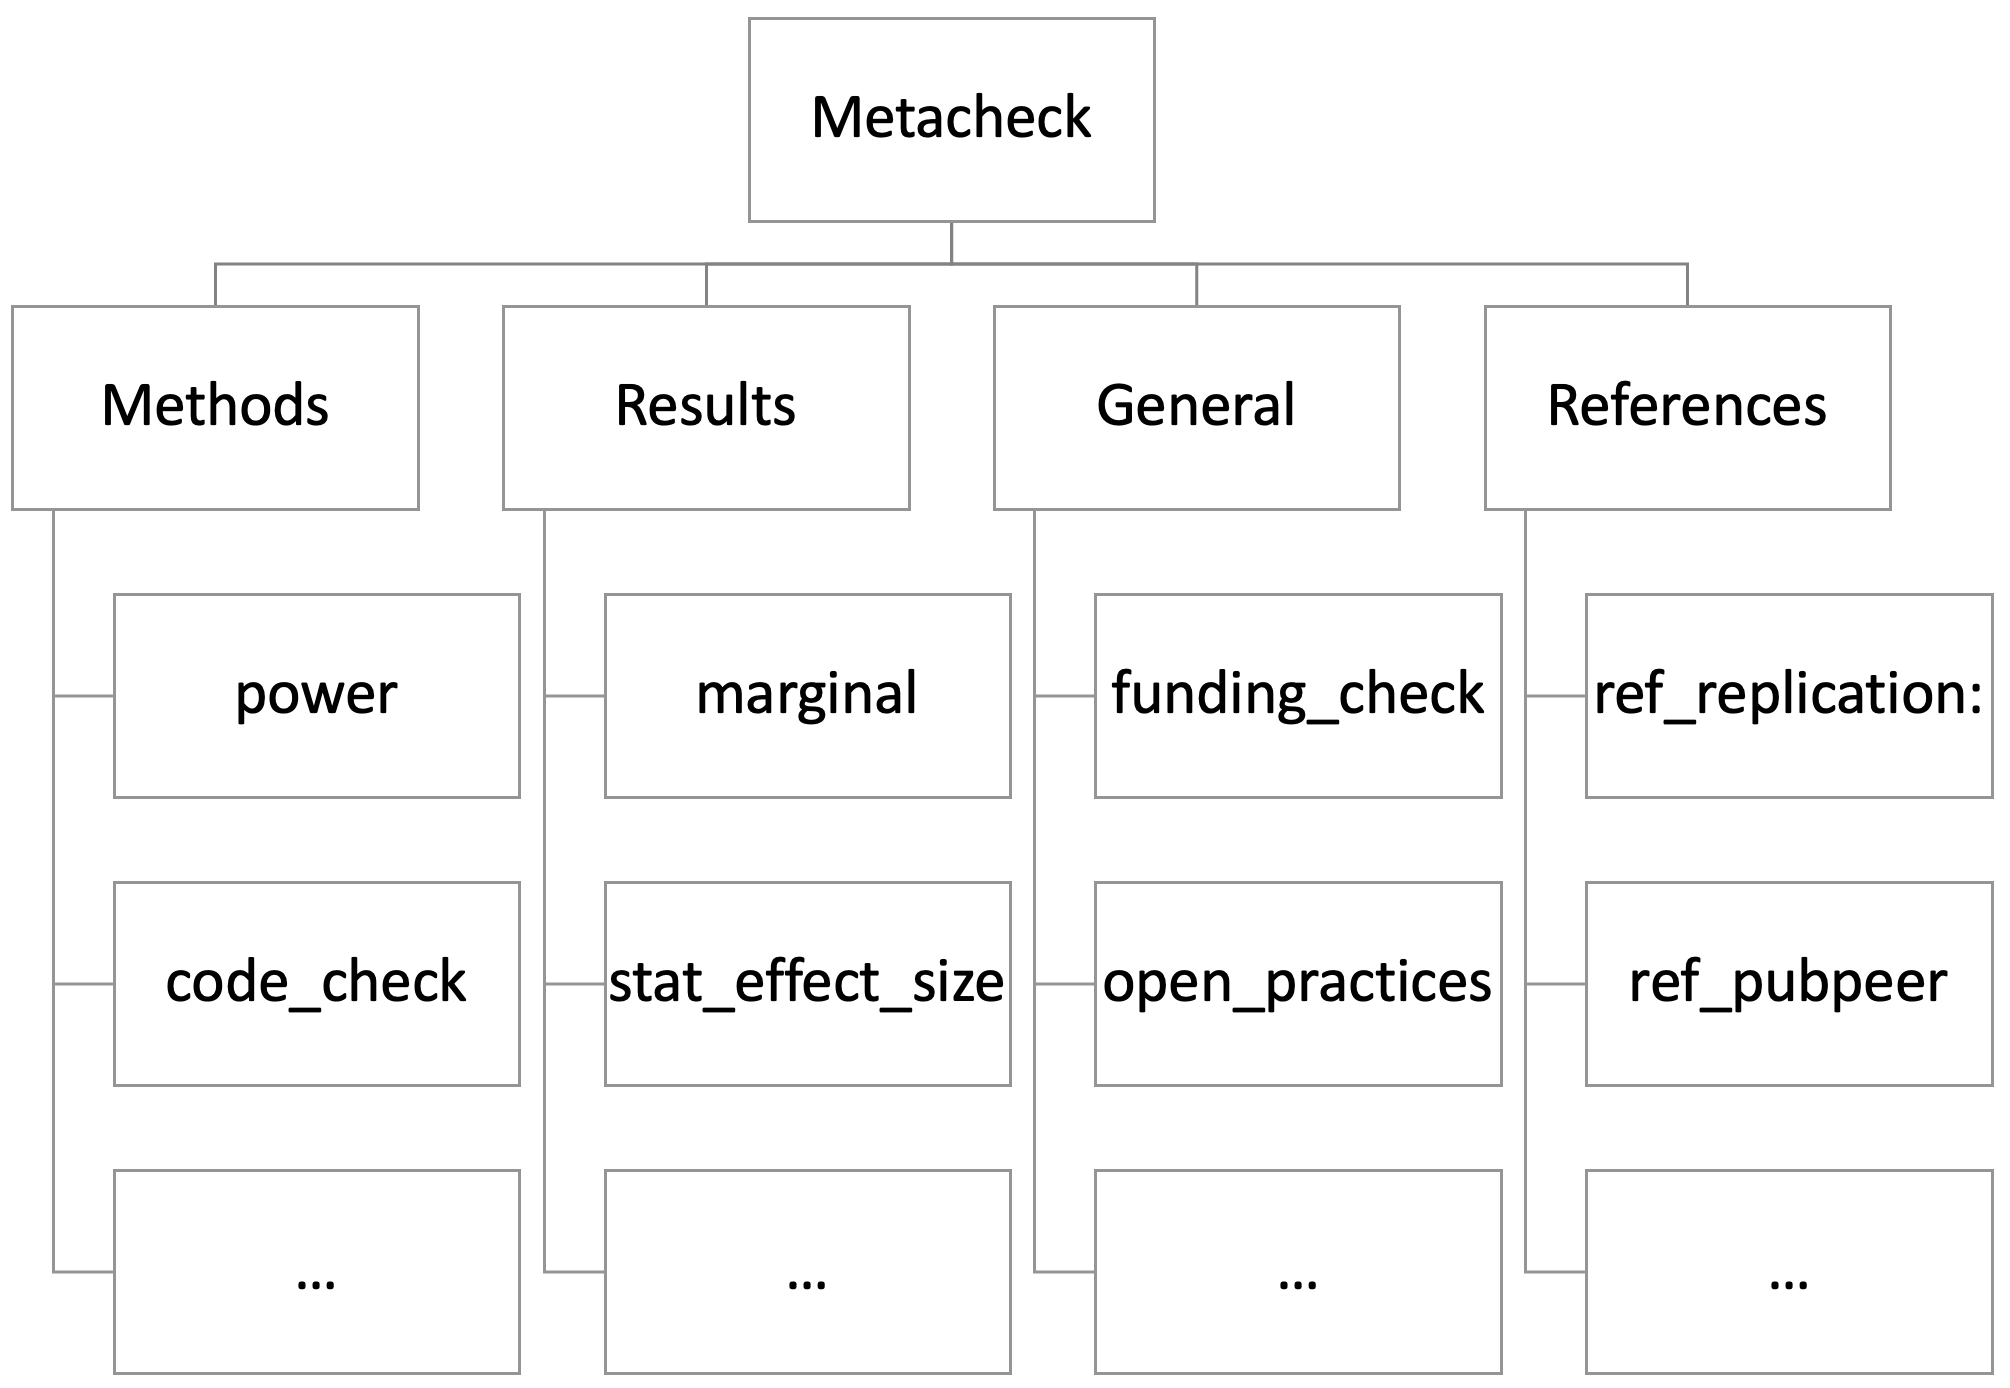
\includegraphics[width=0.8\linewidth]{figures/modules} \end{center}
\end{frame}

\begin{frame}[fragile]{code\_check}
\protect\phantomsection\label{code_check}
\begin{Shaded}
\begin{Highlighting}[]
\FunctionTok{library}\NormalTok{(metacheck)}
\CommentTok{\# psychsci is an built{-}in dataset of 250 open access papers from Psychological Science}

\NormalTok{(res }\OtherTok{\textless{}{-}} \FunctionTok{module\_run}\NormalTok{(psychsci[[}\DecValTok{250}\NormalTok{]], }\StringTok{"code\_check"}\NormalTok{))}
\end{Highlighting}
\end{Shaded}

\begin{verbatim}
## Code Check: 
## -  We found 2 R, SAS, SPSS, or Stata code files.
## -  All your code files had comments.
## -  All files loaded in the code were present in the repository.
## -  No absolute file paths were found.
## -  All libraries/imports were loaded in one block.
\end{verbatim}
\end{frame}

\begin{frame}[fragile]{marginal}
\protect\phantomsection\label{marginal}
\begin{verbatim}
## Marginal Significance: You described 0 effects with terms related to 'marginally significant'.
\end{verbatim}
\end{frame}

\begin{frame}[fragile]{stat\_effect\_size}
\protect\phantomsection\label{stat_effect_size}
\begin{verbatim}
##            paper_id ttests_with_es ttests_without_es Ftests_with_es
## 1 09567976241279291              2                 1              0
##   Ftests_without_es
## 1                 0
\end{verbatim}

\begin{verbatim}
## # A tibble: 3 x 8
##   paper_id          text   section_id paragraph_id text_id es    test_text test 
##   <chr>             <chr>       <int>        <int>   <int> <chr> <chr>     <chr>
## 1 09567976241279291 Neith~         13           43     208 <NA>  t(19) = ~ t-te~
## 2 09567976241279291 The a~         14           47     219 Cohe~ t(19) = ~ t-te~
## 3 09567976241279291 The d~         14           47     222 Cohe~ t(19) = ~ t-te~
\end{verbatim}
\end{frame}

\begin{frame}[fragile]{power}
\protect\phantomsection\label{power}
\begin{verbatim}
## Power Analysis Check: We detected 1 potential power analysis.
\end{verbatim}

\begin{verbatim}
## # A tibble: 1 x 11
##   text_id paragraph_id section_id text  page_number paper_id header section_type
##   <lgl>          <int>      <int> <chr> <lgl>       <chr>    <chr>  <chr>       
## 1 NA                24          6 We c~ NA          0956797~ Parti~ method      
## # i 3 more variables: power_type <chr>, complete <lgl>, power_id <int>
\end{verbatim}
\end{frame}

\end{document}
